\documentclass[10pt,spanish,aspectratio=1610]{beamer}
\usepackage[utf8]{inputenc}
\usepackage{amsmath}
\usepackage{graphicx}
\usepackage{amssymb}
\usepackage{multicol}
\usepackage[spanish]{babel}
\spanishdecimal{.}
\usepackage{subfig}
\usepackage{fancyhdr}
\usepackage{pstricks}
\usepackage{color}
\usepackage[ruled]{algorithm2e}
\usepackage{listings}
\usepackage{xcolor}
\usepackage{gensymb}

\definecolor{graywhite}{rgb}{0.9529,0.9607,0.9686}
\definecolor{bluegray}{rgb}{0.6823, 0.7411, 0.8}
\definecolor{darkred}{rgb}{0.7372, 0.2392, 0.2392}
\definecolor{bluedark}{rgb}{0.294, 0.4705, 0.6407}
\definecolor{darkgreen}{rgb}{0.1764, 0.5294, 0.0901}
\lstset{
  backgroundcolor=\color{graywhite},   % choose the background color; you must add \usepackage{color} or \usepackage{xcolor}; should come as last argument
  basicstyle=\footnotesize,        % the size of the fonts that are used for the code
  breakatwhitespace=false,         % sets if automatic breaks should only happen at whitespace
  breaklines=true,                 % sets automatic line breaking
  captionpos=b,                    % sets the caption-position to bottom
  commentstyle=\color{darkgreen},    % comment style
  keepspaces=true,                 % keeps spaces in text, useful for keeping indentation of code (possibly needs columns=flexible)
  keywordstyle=\color{darkred},       % keyword style
  language=Octave,                 % the language of the code
  morekeywords={*,...},            % if you want to add more keywords to the set
  numbers=left,                    % where to put the line-numbers; possible values are (none, left, right)
  numbersep=7pt,                   % how far the line-numbers are from the code
  numberstyle=\tiny\color{bluedark}, % the style that is used for the line-numbers
  showspaces=false,                % show spaces everywhere adding particular underscores; it overrides 'showstringspaces'
  showstringspaces=false,          % underline spaces within strings only
  showtabs=false,                  % show tabs within strings adding particular underscores
  stepnumber=1,                    % the step between two line-numbers. If it's 1, each line will be numbered
  stringstyle=\color{bluedark},     % string literal style
  frame=single,
  rulecolor=\color{bluegray},
  tabsize=2,                   % sets default tabsize to 2 spaces
  xleftmargin=1cm,
  xrightmargin=0.5cm,
  framexleftmargin=0.5cm,
  extendedchars=true,
  literate={á}{{\'a}}1 {é}{{\'e}}1 {í}{{\'i}}1 {ó}{{\'o}}1 {ú}{{\'u}}1 {Á}{{\'A}}1 {É}{{\'E}}1 {Í}{{\'I}}1 {Ó}{{\'O}}1 {Ú}{{\'U}}1,
}

\DeclareMathOperator{\atantwo}{atan2}
\setbeamercolor{block title}{fg=white,bg=blue!70!black}
\setbeamercolor{block body}{fg=black, bg=blue!10!white}
\setbeamertemplate{blocks}[rounded][shadow=false]
\setbeamercovered{transparent}
\beamertemplatenavigationsymbolsempty
\setbeamertemplate{frametitle}{
  \leavevmode
  \hbox{\begin{beamercolorbox}[wd=0.85\paperwidth,left]{frametitle}
    \usebeamerfont{frametitle}\insertframetitle
  \end{beamercolorbox}
%  \begin{beamercolorbox}[wd=0.25\paperwidth,center]{frametitle}
%    \usebeamerfont{frametitle}\hfill\hspace*{5ex}\footnotesize{\insertsubsection}
%  \end{beamercolorbox}
}}
\setbeamertemplate{footline}{
  \leavevmode%
  \hbox{%
    \begin{beamercolorbox}[colsep=-0.5pt,wd=.33\paperwidth,ht=3ex,dp=1.5ex,center]{author in head/foot}%
      \usebeamerfont{author in head/foot}\insertshortauthor~~ (\insertshortinstitute)
    \end{beamercolorbox}%
    \begin{beamercolorbox}[colsep=-0.5pt,wd=.34\paperwidth,ht=3ex,dp=1.5ex,center]{date in head/foot}%
      \usebeamerfont{author in head/foot}\insertshorttitle
    \end{beamercolorbox}%
    \begin{beamercolorbox}[colsep=-0.5pt,wd=.33\paperwidth,ht=3ex,dp=1.5ex,right]{author in head/foot}%
      \usebeamerfont{author in head/foot}\insertsection{}\hspace*{2em}\scriptsize{\insertframenumber{}}\hspace*{1ex}
    \end{beamercolorbox}
  }
}
\setbeamersize
{
    text margin left=0.25cm,
    text margin right=0.25cm
}

\begin{document}
\renewcommand{\tablename}{Tabla}
\renewcommand{\figurename}{Figura}

\title[Arduino y ROS]{Utilización del entorno ROS y sensores utilizando Arduino}
\author[Dr. Marco Negrete]{Dr. Marco Negrete}
\institute[FI, UNAM]{Facultad de Ingeniería, UNAM}
\date[5to CNIME - 2023]{5to Congreso Nacional de Ingeniería Mecánica Eléctrica\\Universidad Juárez Autónoma de Tabasco\\Agosto de 2023}

\begin{frame}
\titlepage
\end{frame}

%%%%%%%%%%%%%%%%%%%
%%% 2023-08-22 %%%%
%%%%%%%%%%%%%%%%%%%
\section{La plataforma ROS (2023-08-22)}
\begin{frame}\frametitle{La plataforma ROS}
  
\includegraphics[width=0.3\textwidth]{Figures/Ros_logo.png}
  \[\]
  \textbf{ROS (Robot Operating System) } es un \textit{middleware} de código abierto para el desarrollo de robots móviles.
  \begin{itemize}
  \item Implementa funcionalidades comúnmente usadas en el desarrollo de robots como el paso de mensajes entre procesos y la administración de paquetes.
  \item Muchos drivers y algoritmos ya están implementados.
  \item Es una plataforma distribuida de procesos (llamados \textit{nodos}).
  \item Facilita el reuso de código.
  \item Independiente del lenguaje (Python y C++ son los más usados).
  \item Facilita el escalamiento para proyectos de gran escala. 
  \end{itemize}
\end{frame}

\begin{frame}\frametitle{Conceptos}
  ROS se puede entender en dos grandes niveles conceptuales:
  \begin{itemize}
  \item \textbf{Sistema de archivos:} Recursos de ROS en disco
  \item \textbf{Grafo de procesos:} Una red \textit{peer-to-peer} de procesos (llamados nodos) en tiempo de ejecución.
  \end{itemize}
\end{frame}

\begin{frame}\frametitle{Sistema de archivos}
  \begin{columns}
    \begin{column}{0.5\textwidth}
      Recursos en disco:
      \begin{itemize}
      \item \textbf{Workspace:} carpeta que contiene los paquete desarrollados
      \item \textbf{Paquetes:} Principal unidad de organización del software en ROS (concepto heredado de Linux)
      \item \textbf{Manifiesto:} (\texttt{package.xml}) provee metadatos sobre el paquete (dependencias, banderas de compilación, información del desarrollador)
      \item \textbf{Mensajes (msg):} Archivos que definen la estructura de un \textit{mensaje} en ROS.
        \item \textbf{Servicios (srv):} Archivos que definen las estructuras de la petición (\textit{request}) y respuesta (\textit{response}) de un servicio. 
      \end{itemize}
    \end{column}
    \begin{column}{0.4\textwidth}
      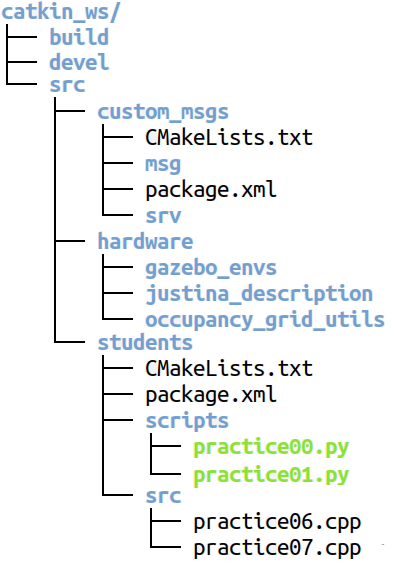
\includegraphics[width=\textwidth]{Figures/catkin_tree.png}
    \end{column}
  \end{columns}
\end{frame}

\begin{frame}\frametitle{Grafo de procesos}
  El grafo de procesos es una red \textit{peer-to-peer} de programas (nodos) que intercambian información entre sí. Los principales componentes del este grafo son:
  \[\]
  \begin{columns}
    \begin{column}{0.5\textwidth}
      \begin{itemize}
      \item master
      \item servidor de parámetros
      \item nodos
      \item mensajes
      \item servicios 
      \end{itemize}
    \end{column}
    \begin{column}{0.5\textwidth}
      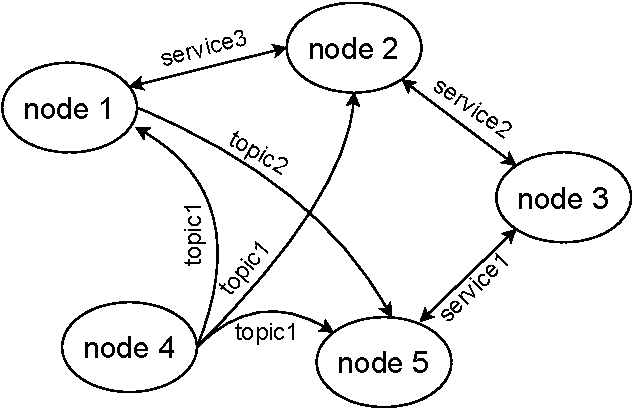
\includegraphics[width=\textwidth]{Figures/RosGraph.pdf}
    \end{column}
  \end{columns}
\end{frame}

\begin{frame}\frametitle{Tópicos y servicios}
  Los nodos (procesos) en ROS intercambian información a través de dos grandes patrones:
  \begin{columns}
    \begin{column}{0.6\textwidth}
        \begin{itemize}
        \item \textbf{Tópicos}
          \begin{itemize}
          \item Son un patrón $1:n$ de tipo \textit{publicador/suscriptor}
          \item Son no bloqueantes
          \item Utilizan estructuras de datos definidas en archivos \texttt{*.msg} para el envío de información
          \end{itemize}
        \item \textbf{Servicios}
          \begin{itemize}
          \item Son un patrón $1:1$ de tipo \textit{petición/respuesta}
          \item Son bloqueantes
          \item Utilizan estructuras de datos definidas en archivos \texttt{*.srv} para el intercambio de información. 
          \end{itemize}
        \end{itemize}
    \end{column}
    \begin{column}{0.4\textwidth}
      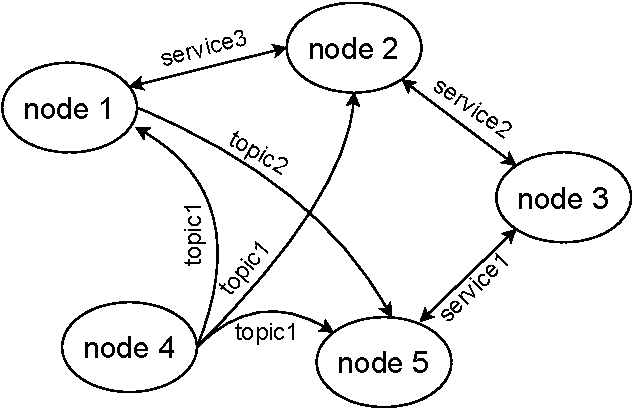
\includegraphics[width=\textwidth]{Figures/RosGraph.pdf}
    \end{column}
  \end{columns}
  \[\]
  Para mayor información:
  \begin{itemize}
  \item Tutoriales \url{http://wiki.ros.org/ROS/Tutorials}
  \item Koubâa, A. (Ed.). (2020). Robot Operating System (ROS): The Complete Reference. Springer Nature
  \end{itemize}
\end{frame}

\begin{frame}\frametitle{El simulador Gazebo}
  \begin{itemize}
  \item Es un simulador basado en el motor ODE
  \item Permite simular los sensores y actuadores más comunes en robots móviles:
    \begin{itemize}
    \item Cámaras RGB 
    \item Cámaras RGB-D
    \item Sensores Lidar
    \item Encoders
    \item Motores y reducciones
    \item Bases móviles 
    \end{itemize}
  \item Ya tiene \textit{plugins} para interactuar con ROS
  \end{itemize}
\end{frame}

\begin{frame}
  \Large{Contacto}
  \[\]
  \large
  Dr. Marco Negrete\\
  Profesor Asociado C\\
  Departamento de Procesamiento de Señales\\
  Facultad de Ingeniería, UNAM.
  \[\]
  marco.negrete@ingenieria.unam.edu\\
\end{frame}
\end{document}
